\documentclass[../main.tex]{subfiles}
\begin{document}
\chapter{Wind parameter spaces}\label{appendix_errospaces}
In Section \ref{section:wind_rootfinding}, we showed the boundary condition errors on the ($\Edot$,$T_c$) parameter space for the $\Mdot=10^{18.5}$ g s$^{-1}$ wind. It is useful for potential future work to examine these parameter spaces at other values of the mass-loss rate. 

Starting at $10^{18}$ g s$^{-1}$, we often encountered an interesting problem in the outer integration, represented by the purple dots in the figures below. Before approaching a photosphere, the velocity of the gas began decreasing and eventually approached the sound speed. This causes divergences in our equations, so we had to stop the integrations. Concurrent with the decreasing velocity, the density of the gas increased outward, indicating the formation of a shell. Investigating these solutions would require improvements in the model and more flexible boundary conditions. Most likely however, a proper analysis would involve time-dependent calculations.

In the inwards integration, we found that for large regions of the parameter space, shown by the green dots in the figures below, we could never hit the required column depth of $10^8$ g cm$^{-2}$ for the boundary condition, as the integration would strongly diverge at lower pressures. We were not able to find a physical explanation for these divergences.


\begin{figure}[ht!]
    \centering
    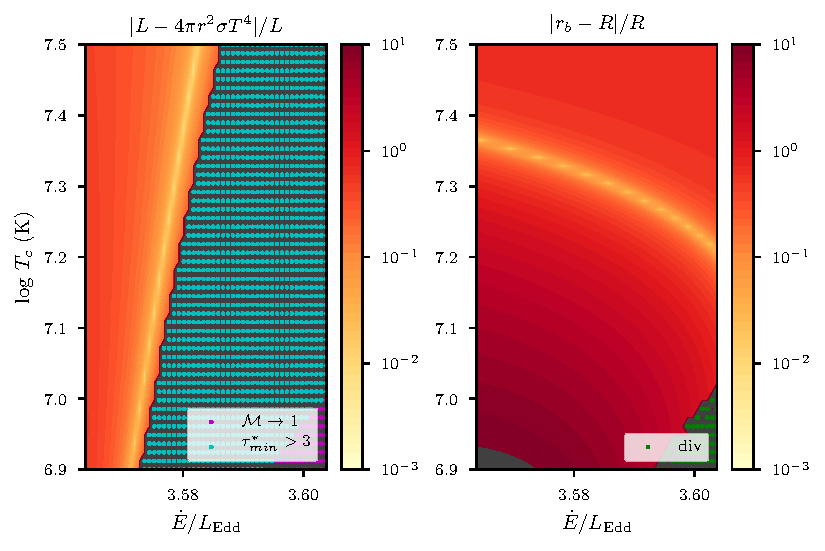
\includegraphics[width=0.8\textwidth]{figures/errorspace_18.pdf}
    \vspace*{-0.5cm}
    % \caption[B.C. errors on the $\log\dot{M}=18$ wind parameter space]{Boundary condition errors on the $\log\dot{M}=\bm{18}$ parameter space.}
    \caption*{Boundary condition errors on the $\log\dot{M}=\bm{18}$ parameter space.}
    \label{fig:errorspace_18}
\end{figure}

\begin{figure}[ht!]
    \centering
    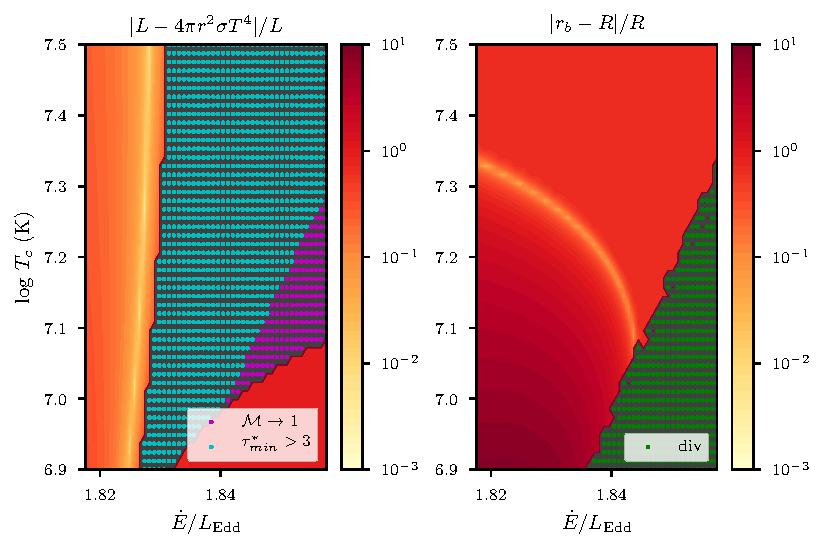
\includegraphics[width=0.8\textwidth]{figures/errorspace_17_5.pdf}
    \vspace*{-0.5cm}
    % \caption[B.C. errors on the $\log\dot{M}=17.5$ wind parameter space]{Boundary condition errors on the $\log\dot{M}=\bm{17.5}$ parameter space.}
    \caption*{Boundary condition errors on the $\log\dot{M}=\bm{17.5}$ parameter space.}
    \label{fig:errorspace_17_5}
\end{figure}

\begin{figure}[h!]
    \centering
    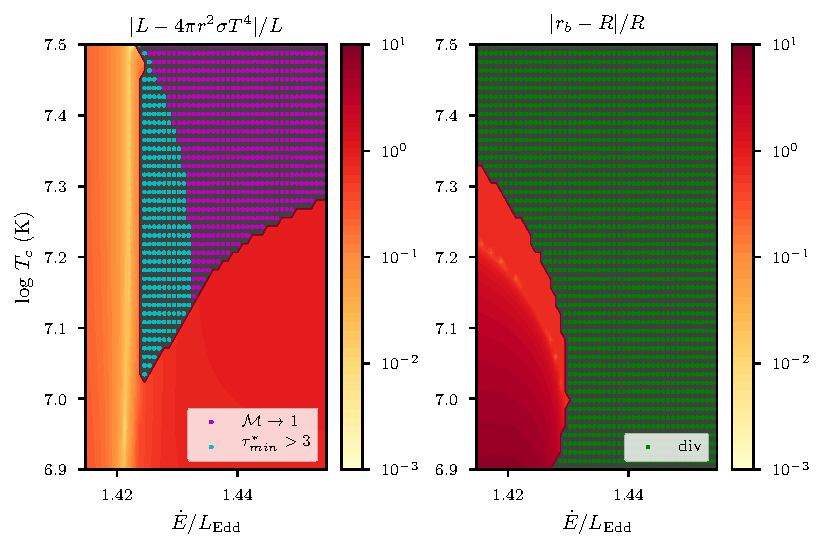
\includegraphics[width=0.8\textwidth]{figures/errorspace_17_2.pdf}
    \vspace*{-0.5cm}
    % \caption[B.C. errors on the $\log\dot{M}=17.2$ wind parameter space]{Boundary condition errors on the $\log\dot{M}=\bm{17.2}$ parameter space.}
    \caption*{Boundary condition errors on the $\log\dot{M}=\bm{17.2}$ parameter space.}
    \label{fig:errorspace_17_2}
\end{figure}


\end{document}
